\documentclass[crop,tikz]{standalone}
\begin{document}
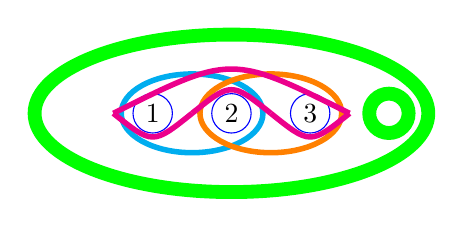
\begin{tikzpicture}
  \draw (-1,0) node{1};
  \draw (0,0) node{2};
  \draw (1,0) node{3};
  \draw[green, line width=5] (0,0) circle [ x radius = 2.5, y radius = 1];

  \draw[blue] (-1,0) circle [x radius =.25, y radius = .25];
  \draw[blue] (0,0) circle [x radius =.25, y radius = .25];
  \draw[blue] (1,0) circle [x radius =.25, y radius = .25];

  \draw[cyan, line width=2pt] (-.5,0) circle [x radius =.9, y radius = .5];
  \draw[orange, line width=2pt] (0.5,0) circle [x radius =.9, y radius = .5];

  \draw[magenta, line width=2pt] (-1.5,0) .. controls (0,.75) .. (1.5,0);
  \draw[magenta, line width=2pt] (-1.5,0) .. controls (-1, -.4) .. (-.5,0);
  \draw[magenta, line width=2pt] (-.5,0) .. controls (0,.4) .. (.5,0);
  \draw[magenta, line width=2pt] (.5,0) .. controls (1,-.4) .. (1.5,0);

  \draw[green, line width=5] (2,0) circle [x radius =.25, y radius = .25];
\end{tikzpicture}
\end{document}
